\documentclass[a4paper,fleqn]{cas-sc}
% \documentclass[a4paper,fleqn]{cas-dc}

%\usepackage[authoryear,longnamesfirst]{natbib}
%\usepackage[authoryear]{natbib}
\usepackage{array}
\usepackage{tabularx}
\usepackage[numbers]{natbib}
\usepackage{bm}
\usepackage{amsfonts} 
\usepackage{dsfont}
\usepackage{graphicx}
\usepackage{xcolor}
\usepackage{subcaption}
\usepackage{booktabs}
\usepackage{placeins}
\usepackage{tikz}
\usepackage{float}
\usepackage{flafter}
\usepackage{afterpage}

\renewcommand{\topfraction}{0.9}
\renewcommand{\bottomfraction}{0.8}
\renewcommand{\textfraction}{0.07}
\renewcommand{\floatpagefraction}{0.75}

\setcounter{topnumber}{3}
\setcounter{bottomnumber}{2}
\setcounter{totalnumber}{5}
\usetikzlibrary{
    arrows.meta,
    positioning,
    calc,
    shapes.geometric,
    fit,
    backgrounds
}

% Workflow colors
\definecolor{wfBlue}{RGB}{47,111,178}
\definecolor{wfBlueDark}{RGB}{30,78,125}
\definecolor{wfBlueLight}{RGB}{235,244,252}

\definecolor{wfTeal}{RGB}{39,153,146}
\definecolor{wfTealDark}{RGB}{25,105,100}
\definecolor{wfTealLight}{RGB}{234,248,246}

\definecolor{wfOrange}{RGB}{230,145,45}
\definecolor{wfOrangeDark}{RGB}{176,101,20}
\definecolor{wfOrangeLight}{RGB}{253,243,229}

\definecolor{wfPurple}{RGB}{116,91,166}
\definecolor{wfPurpleDark}{RGB}{79,58,126}
\definecolor{wfPurpleLight}{RGB}{244,240,250}

\definecolor{wfGray}{RGB}{100,100,100}% Gray for citation box borders
%%%Author definitions
\def\tsc#1{\csdef{#1}{\textsc{\lowercase{#1}}\xspace}}
\tsc{WGM}
\tsc{QE}
\tsc{EP}
\tsc{PMS}
\tsc{BEC}
\tsc{DE}
%%%

\begin{document}
\let\WriteBookmarks\relax
\shorttitle{Patent and Policy Impact of ML for OPF}
\shortauthors{M.D.A. Firdausi, M.F. Muna, M.N. Syed, A.I. Malik, and S. Riaz}

\title [mode = title]{From Academic Research to Technological and Policy Impact: A Comparative Analysis of Patent- and Policy-Cited Machine Learning for Optimal Power Flow}
% \tnotemark[1,2]

% \tnotetext[1]{This document is the results of the research project funded by the National Science Foundation.}

% \tnotetext[2]{The second title footnote which is a longer text matter to fill through the whole text width and overflow into another line in the footnotes area of the first page.}

\author[1]{Muhammad Dzulqarnain Al Firdausi}[
                        % type=editor,
                        % auid=000,bioid=1,
                        % prefix=Sir,
                        % role=Researcher,
                        orcid=0000-0002-2794-0970]
% \cormark[1]
% \fnmark[1]
% \ead{g202210120@kfupm.edu.sa}
% \ead[url]{www.jkkrishnan.in}

\credit{Conceptualization, methodology, software, formal analysis, writing original draft preparation}

%\address[1]{, Street 129, 1043 NX Amsterdam, The Netherlands}
\affiliation[1]{organization={Industrial and Systems Engineering Department, King Fahd University of Petroleum and Minerals},
                % addressline={Jawahar Nagar}, 
                city={Dhahran},
%               citysep={}, % Uncomment if no comma needed between city and postcode
                postcode={31261}, 
                % state={Kerala},
                country={Saudi Arabia}}

\author[1]{M Fahrudin Muna}[
                        % type=editor,
                        % auid=000,bioid=1,
                        % prefix=Sir,
                        % role=Researcher,
                        orcid=0000-0002-8236-3520]
% \cormark[1]
% \fnmark[1]
% \ead{g202210120@kfupm.edu.sa}
% \ead[url]{www.jkkrishnan.in}

\credit{Conceptualization, methodology, software, formal analysis, writing original draft preparation}

%\address[1]{, Street 129, 1043 NX Amsterdam, The Netherlands}
\affiliation[1]{organization={Industrial and Systems Engineering Department, King Fahd University of Petroleum and Minerals},
                % addressline={Jawahar Nagar}, 
                city={Dhahran},
%               citysep={}, % Uncomment if no comma needed between city and postcode
                postcode={31261}, 
                % state={Kerala},
                country={Saudi Arabia}}

\author[1,2,3]{Mujahid N. Syed}[
                        % type=editor,
                        % auid=000,bioid=1,
                        % prefix=Sir,
                        % role=Researcher,
                        orcid=0000-0002-3862-2935]
\cormark[1]
\ead{smujahid@kfupm.edu.sa, snumujahid@gmail.com}
\credit{Conceptualization, methodology, validation, formal analysis, investigation, writing original draft preparation, writing review and editing, supervision, project administration}
\cortext[cor1]{Corresponding author}

\affiliation[2]{organization={Interdisciplinary Research Center for Intelligent Secure Systems, King Fahd University of Petroleum and Minerals},
                % addressline={Street 29}, 
                postcode={31261}, 
                % postcodesep={}, 
                city={Dhahran},
                country={Saudi Arabia}}


\affiliation[3]{organization={Joint Research Center for Artificial Intelligence, King Fahd University of Petroleum and Minerals},
                % addressline={Street 29}, 
                postcode={31261}, 
                % postcodesep={}, 
                city={Dhahran},
                country={Saudi Arabia}}

\author[1,2,4]{Asif Iqbal Malik}[
                        % type=editor,
                        % auid=000,bioid=1,
                        % prefix=Sir,
                        % role=Researcher,
                        orcid=0000-0002-9607-6530]
% \cormark[1]
% \fnmark[2]
% \ead[URL]{https://www.university.org}

\credit{Conceptualization, methodology, validation, formal analysis, investigation, writing original draft preparation, writing review and editing, supervision, project administration}

\affiliation[4]{organization={IRC for Smart Mobility and Logistics, King Fahd University of Petroleum and Minerals},
                % addressline={Street 29}, 
                postcode={31261}, 
                % postcodesep={}, 
                city={Dhahran},
                country={Saudi Arabia}}

\author[5]{Shahina Riaz}[
                        % type=editor,
                        % auid=000,bioid=1,
                        % prefix=Sir,
                        % role=Researcher,
                        orcid=0000-0002-6695-4283]
% \cormark[1]
% \fnmark[2]
% \ead[URL]{https://www.university.org}

\credit{Methodology, validation}

\affiliation[5]{organization={IRC for Refining and Advanced Chemicals, King Fahd University of Petroleum and Minerals},
                % addressline={Street 29}, 
                postcode={31261}, 
                % postcodesep={}, 
                city={Dhahran},
                country={Saudi Arabia}}

% \cortext[cor2]{Principal corresponding author}
% \fntext[fn1]{This is the first author footnote, but is common to third author as well.}
% \fntext[fn2]{Another author footnote, this is a very long footnote and it should be a really long footnote. But this footnote is not yet  sufficiently long enough to make two lines of footnote text.}

% \nonumnote{This note has no numbers. In this work we demonstrate $a_b$ the formation Y\_1 of a new type of polariton on the interface between a cuprous oxide slab and a polystyrene micro-sphere placed on the slab. }

\begin{abstract}
Machine learning (ML) and optimisation increasingly support optimal power flow (OPF), yet scholarly influence alone does not reveal which research themes attract technological and policy attention. This study combines bibliometric analysis and semantic topic modelling to compare the academic, patent-cited, and policy-cited ML--OPF literature. A DOI-linked population of 15,857 Scopus publications was matched with patent citations from Lens and policy citations from Overton. Independently selected BERTopic models identified 18 academic, 16 patent-cited, and nine policy-cited topics, with LDA providing reference partitions. Patent citations reached 778 publications (4.91\%), while policy citations reached 392 (2.47\%); only 83 publications appeared in both collections. Patent coverage was broader, whereas policy-cited publications received more external citations per cited publication. Topic-level comparisons showed stronger patent representation for reinforcement learning and neural OPF methods, while smart-energy management and grid resilience exhibited greater policy coverage. Distributed optimisation connected multiple topics across both pathways. Temporal analysis indicated increasing shares of graph and physics-informed learning and reinforcement learning, alongside declining relative shares of established distributed and metaheuristic optimisation themes. The reviewed literature motivates further work on physical feasibility, generalisation, uncertainty-aware decisions, communication constraints, and realistic operational validation. These findings demonstrate the value of examining patent and policy citations as complementary indicators of external research attention. They describe citation linkages rather than implementation or causal impact and remain subject to database coverage, retrieval scope, and unequal citation windows.
\end{abstract}

% \begin{graphicalabstract}
% \includegraphics{figs/cas-grabs.pdf}
% \end{graphicalabstract}

% \begin{highlights}
% \item Research highlights item 1
% \item Research highlights item 2
% \item Research highlights item 3
% \end{highlights}

\begin{keywords}
Optimal power flow \sep Machine learning \sep Power-system optimisation \sep BERTopic \sep Bibliometric analysis \sep Patent citations \sep Policy citations
\end{keywords}

\maketitle
\section{Introduction}
\label{sec:introduction}

\subsection{Optimal Power Flow in the Energy Transition}

Power systems increasingly incorporate renewable generation, distributed energy resources (DERs), storage, and flexible demand. These developments support decarbonization but introduce uncertainty, changing power-flow patterns, and greater coordination requirements. Optimal Power Flow (OPF) supports operational and planning decisions by optimizing objectives such as generation cost, network losses, or environmental performance while satisfying power-flow equations and engineering limits. Its applications extend from generation dispatch to transmission planning, renewable integration, and cross-border electricity exchanges \cite{singh2014optimal}. Probabilistic formulations further address uncertain and correlated loads and renewable production, connecting operational optimization with reliability and investment concerns \cite{aien2015probabilistic}.

The expansion of smart grids and microgrids has broadened OPF research to include distributed generation, storage, demand response, voltage regulation, and multi-objective decision-making \cite{abdi2017review}. Islanded microgrids introduce additional challenges involving frequency variation, generator control modes, and power sharing \cite{moradi2017power}. Meanwhile, behind-the-meter resources and decentralized electricity trading connect network-constrained optimization with transactive energy, virtual power plants, and consumer participation \cite{guerrero2020towards}.

These applications have encouraged diverse computational approaches, including metaheuristics for nonconvex and mixed-variable problems \cite{papadimitrakis2021metaheuristic}, distributed optimization, and machine learning (ML). ML can accelerate optimization through predictions based on previous solutions, while optimization can improve the feasibility of learned decisions \cite{steven2026machine}. This methodological and application diversity raises a broader question: which areas of the OPF knowledge base attract attention from technological and policy communities?

\subsection{Patent and Policy Citations as Complementary Impact Signals}

Publication counts and scholarly citations describe academic activity but offer limited insight into how research enters technological and institutional knowledge bases. Patent citations identify scholarly publications referenced in documents associated with inventions, whereas policy citations identify publications referenced by governments, regulators, intergovernmental organizations, and other policy-oriented institutions. These pathways provide complementary evidence of non-academic attention. However, neither establishes implementation, commercialization, policy adoption, or causal impact.

This distinction is particularly relevant to OPF, which connects computational methods with grid technologies, electricity markets, reliability, and renewable integration. Different research themes may attract different levels of patent and policy attention. Existing reviews classify OPF formulations, algorithms, and applications, but provide less insight into whether patent-cited and policy-cited publications represent similar or distinct parts of this knowledge base. Comparing both pathways against the academic literature can reveal themes that receive relatively greater technological attention, institutional attention, or attention across both domains.

Accordingly, this study examines which topics characterize the academic, patent-cited, and policy-cited ML--OPF literature; which themes are shared or differently represented across these corpora; and how their prevalence changes over time. These questions concern documented knowledge uptake rather than demonstrated technological or policy outcomes.

\subsection{Contributions and Paper Organization}
\label{sec:contributions_outline}

The study links a Scopus academic corpus with patent citations identified through Lens and policy citations identified through Overton. BERTopic is applied separately to the three corpora to identify semantic clusters, whose interpretations are supported by representative terms and publications. Cross-corpus thematic harmonization provides a common basis for comparing topic prevalence and tracing patent- and policy-cited publications to the broader academic literature.

The contributions are threefold. First, the study integrates academic, technological, and policy citation perspectives within a comparative framework for ML--OPF research. Second, it combines semantic topic modeling with citation linkage to identify shared and distinctive research themes beyond aggregate citation counts. Third, it examines thematic development and differences in external attention to inform discussion of research translation opportunities for researchers, technology developers, system operators, and policymakers.

% Section~\ref{sec:methodology} describes corpus construction, preprocessing, BERTopic modeling, and thematic harmonization. Section~\ref{sec:academic_landscape} characterizes the academic baseline, and Section~\ref{sec:citation_comparison} examines patent and policy citation patterns. Section~\ref{sec:topic_analysis} compares thematic structures across the three corpora. Section~\ref{sec:translation_opportunities} discusses translation opportunities, and Section~\ref{sec:conclusions} presents limitations and conclusions.

\section{Research Design and Methods}\label{sec:methodology}

This study compares latent Dirichlet allocation (LDA), BERTopic, and an LDA--BERTopic hybrid to examine the thematic structure of machine-learning-related optimal power flow (OPF) research and its citation links to patents and policy documents. Three scholarly corpora are analysed: the Scopus research corpus, its patent-cited subset identified through Lens, and its policy-cited subset identified through Overton. Models are estimated separately for each corpus, while normalized Digital Object Identifiers (DOIs) connect publications across the three layers.

\begin{figure}
    \centering
    \includegraphics[width=0.5\linewidth]{figs/opf_workflow.pdf}
    \caption{OPF research workflow integrating LDA, BERTopic and hybrid topic modelling across the Scopus academic corpus and its Lens patent-cited and Overton policy-cited subsets. Corpus counts distinguish model estimation from the common scope used for pathway analysis.}
    \label{fig:research_workflow}
\end{figure}

\subsection{Data Collection and Corpus Definition}\label{sec:corpus_construction}

English-language publications were retrieved using the Scopus \emph{All fields} option with the following search expression:

\begin{quote}
\begin{verbatim}
"Power flow" AND "Machine learning" AND (Optimization OR Optimisation)
AND LIMIT-TO(LANGUAGE, "English")
\end{verbatim}
\end{quote}

This broad search includes matches outside titles, abstracts, and author keywords and can therefore retrieve publications beyond the immediate OPF domain. Exported metadata included publication titles, abstracts, years, authors, source titles, and DOIs.

Scopus DOIs were matched against scholarly works receiving patent citations in Lens and policy-document citations in Overton. The corresponding Scopus titles and abstracts supplied consistent publication text across the datasets. Consequently, Lens and Overton represent citation-selected collections of scholarly publications; the patent and policy documents themselves are not the texts subjected to topic modelling. DOI normalization, duplicate checks, and text preparation produced the modelled populations reported in Table~\ref{tab:opf_corpus_populations}.

\begin{table}[htbp]
\centering
\caption{Bibliometric and topic-modelling populations of the OPF study.}
\label{tab:opf_corpus_populations}
\small
\setlength{\tabcolsep}{6pt}
\renewcommand{\arraystretch}{1.15}
\begin{tabular}{lrrr}
\toprule
Corpus
& \shortstack{DOI-linked\\publications}
& \shortstack{Modelled\\publications}
& \shortstack{Publications\\with a topic} \\
\midrule
Scopus  & 15,857 & 15,743 & 14,904 \\
Lens    & 778    & 777    & 720 \\
Overton & 392    & 390    & 368 \\
\bottomrule
\end{tabular}
\vspace{2mm}
\begin{minipage}{\textwidth}
\footnotesize
\textit{Notes:} DOI-linked counts describe the bibliometric metadata population, while modelled counts refer to the inputs used for topic modelling. Topic-assigned counts are taken from the final BERTopic inventory. Lens and Overton are citation-selected scholarly collections and overlap by 83 publications in the bibliometric population.
\end{minipage}
\end{table}

The thematic analysis uses the final BERTopic assignments, comprising 14,904 Scopus, 720 Lens, and 368 Overton publications with topics. Cross-corpus pathways require a publication to have a topic in both the Scopus model and the corresponding citation-selected model. Consequently, the pathway figure includes 691 Lens publications and 352 Overton publications linked to Scopus topics. These overlap counts differ from the complete topic-assigned populations because they require assignments in both models.

\subsection{Text Representations and LDA Estimation}\label{sec:text_preprocessing}

Readable publication titles and abstracts supplied the inputs to pretrained sentence-embedding models. The combined cleaning pipeline supplied the text used for the LDA reference models. BERTopic topic words were recomputed using c-TF-IDF after outlier reassignment, so the final topic representations corresponded to the evaluated publication assignments.

LDA was estimated independently for each OPF corpus using Gibbs sampling in the R package \texttt{topicmodels}. Table~\ref{tab:opf_lda_parameters} summarizes the topic-number selection and sampling settings reported in the revised-grid appendix, while Table~\ref{tab:opf_lda_parameter_interpretation} explains the modelling parameters.

\begin{table}[htbp]
\centering
\caption{LDA estimation and topic-number selection settings reported for the OPF corpora.}
\label{tab:opf_lda_parameters}
\scriptsize
\setlength{\tabcolsep}{4pt}
\renewcommand{\arraystretch}{1.15}
\begin{tabularx}{\textwidth}{p{30mm}p{39mm}X}
\toprule
Component & Parameter & Reported setting \\
\midrule
Estimation & Software and method & R package \texttt{topicmodels}; Gibbs sampling \\
& Text source & Combined cleaning pipeline \\
& Random seed & 123 \\
\midrule
Validation & Training / held-out split & 80\% / 20\% \\
Topic-number search & Candidate topic numbers & Every integer $K$ from 2 to 25 \\
& Short-chain settings & Burn-in: 50; iterations: 100; thinning: 10 \\
& Candidate proposal & Median of three perplexity-curve readings: rate-of-change point, normalized knee, and diminishing-return threshold \\
\midrule
Candidate checks & Long-chain settings & Burn-in: 500; iterations: 2,000; thinning: 50 \\
& Coherence requirement & Mean UMass coherence within two units of the best neighbouring candidate \\
& Overlap requirement & No pair of topics with topic--word cosine similarity $\geq0.5$ \\
& Retained topic number & Smallest neighbouring candidate satisfying both checks \\
\midrule
Final models & Scopus & $K=10$ \\
& Lens & $K=8$ \\
& Overton & $K=6$ \\
& Check and final chains & Burn-in: 500; iterations: 2,000; thinning: 50 \\
\bottomrule
\end{tabularx}
\vspace{2mm}
\begin{minipage}{\textwidth}
\footnotesize
\textit{Notes:} Settings follow Appendix A of the revised-grid report. The selected LDA models provide the reference topics for the $\kappa_{\mathrm{LDA}}$ criterion. The appendix does not document a separate prior-sensitivity grid, numerical Dirichlet priors, or vocabulary-filtering thresholds; these are therefore not specified in this table.
\end{minipage}
\end{table}

\begin{table}[htbp]
\centering
\caption{Interpretation of LDA parameters and estimation settings.}
\label{tab:opf_lda_parameter_interpretation}
\scriptsize
\setlength{\tabcolsep}{4pt}
\renewcommand{\arraystretch}{1.15}
\begin{tabularx}{\textwidth}{p{31mm}X p{43mm}}
\toprule
Parameter & Meaning & Interpretation \\
\midrule
Number of topics $K$ & Specifies the number of latent word distributions used to describe publications. & Lower values yield broader descriptions; higher values permit finer distinctions and potentially overlapping topics. \\
Document--topic prior $\alpha$ & Controls the concentration of a publication's topic mixture. & Smaller values encourage concentration on fewer topics; larger values encourage more diffuse mixtures. \\
Topic--word prior $\delta$ & Controls the concentration of each topic's word distribution. & Smaller values favour concentrated word distributions; larger values provide stronger smoothing. \\
Burn-in & Initial Gibbs iterations discarded before retained sampling. & Allows the sampler to move away from its initial state; does not itself demonstrate convergence. \\
Subsequent iterations & Sampling iterations performed after burn-in. & Longer runs provide additional sampling but increase computation. \\
Thinning & Interval between retained Gibbs samples. & Larger intervals retain fewer samples for a fixed chain length. \\
Random seed & Controls stochastic initialization and sampling. & A fixed seed supports reproducibility within the computational environment. \\
Training fraction & Proportion of publications used to estimate models during held-out evaluation. & The fixed split supports consistent comparison across candidate settings. \\
Vocabulary filtering & Removes terms with insufficient document or total frequency. & Stricter filtering reduces vocabulary size and can remove rare technical terminology. \\
Dominant-topic assignment & Converts each publication's topic mixture into one topic identifier. & Supports count-based comparisons and DOI-linked pathway construction while discarding mixture information. \\
\bottomrule
\end{tabularx}
\vspace{2mm}
\begin{minipage}{\textwidth}
\footnotesize
\textit{Notes:} Parameter effects are general tendencies. The revised-grid appendix documents topic-number selection and sampling settings but does not specify numerical Dirichlet priors.
\end{minipage}
\end{table}

The held-out perplexity curve was interpreted using three complementary rules: a change in the smoothed marginal improvement, the knee of the normalized curve, and a diminishing-return threshold. The median proposal and its immediate neighbours were refitted using long chains. A candidate passed when its mean UMass coherence was within two units of the best candidate and its maximum pairwise topic--word cosine similarity was below 0.5. The smallest passing value was retained and fitted to the full modelled corpus. For cross-model comparisons and pathway construction, publications received their dominant LDA topic.


\subsection{BERTopic Configuration and Selection}\label{sec:bertopic_modelling}

BERTopic combined pretrained sentence embeddings, UMAP dimensionality reduction, HDBSCAN clustering, and c-TF-IDF topic representations. Models were fitted independently for Scopus, Lens, and Overton. Embeddings were generated from readable publication titles and abstracts and reused across compatible configurations. Table~\ref{tab:opf_bertopic_parameters} summarizes the reported revised search, while Table~\ref{tab:opf_bertopic_parameter_interpretation} explains its parameters and processing controls.

\begin{table}[htbp]
\centering
\caption{BERTopic search space and processing settings in the revised OPF experiment.}
\label{tab:opf_bertopic_parameters}
\scriptsize
\setlength{\tabcolsep}{4pt}
\renewcommand{\arraystretch}{1.15}
\begin{tabularx}{\textwidth}{p{27mm}p{38mm}X}
\toprule
Component & Parameter & Search values or fixed setting \\
\midrule
Sentence embeddings & Embedding model & MiniLM: \texttt{all-MiniLM-L6-v2}; MPNet: \texttt{paraphrase-mpnet-base-v2}; BioBERT-STS: \texttt{BioBERT-mnli-snli-scinli-scitail-mednli-stsb} \\
& Embedded text & Readable publication title and abstract \\
\midrule
UMAP & \texttt{n\_neighbors} & 10, 20, 30, 40, 50, 60 \\
& \texttt{n\_components} & 10, 20, 30, 40, 50, 60 \\
& \texttt{min\_dist} & 0.0 \\
& Distance metric & Cosine \\
& Random seed & 123 \\
\midrule
HDBSCAN & Minimum cluster-size share & 0.5\%, 1.0\%, 1.5\%, 2.0\%, 2.5\%, 3.0\% \\
& Integer conversion & $\max\{10,\operatorname{round}(pN/100)\}$ publications \\
& \texttt{min\_samples} & 10, 20, 30, 40, 50, 60 \\
& Cluster-selection method & Excess of mass (EOM), leaf \\
& Distance metric & Euclidean \\
\midrule
Topic representation & Representation & c-TF-IDF on cleaned unigram stems \\
& Leading terms & Ten terms per topic for lexical evaluation and interpretation \\
\midrule
Concentration controls & Eligible topic count & 5--30 substantive topics \\
& Largest-topic guard & At most 35\% of assigned publications, checked before and after reassignment \\
& Conditional capped refit & Additional EOM fit with a maximum cluster-size setting of 35\% of the corpus when triggered by the initial guard \\
\midrule
Outlier handling & Reassignment criterion & Cosine similarity to a topic centre meeting the threshold derived from the tenth percentile of initial within-topic similarities \\
& Remaining outliers & Retained as an explicit unassigned group \\
\midrule
Experimental design & Base grid per corpus & $3\times6\times6\times6\times6\times2=7{,}776$ configurations \\
& Corpora & Scopus: 15,743; Lens: 777; Overton: 390 modelled publications \\
& Additional configurations & Conditional capped refits, recorded separately from the base grid \\
\bottomrule
\end{tabularx}
\vspace{2mm}
\begin{minipage}{\textwidth}
\footnotesize
\textit{Notes:} Here, $N$ denotes the corresponding modelled corpus size and $p$ denotes the minimum cluster-size percentage. Percentage settings can become equivalent after integer conversion and application of the ten-publication floor, particularly for the smaller corpora. The reported base-grid count refers to nominal parameter combinations. Native HDBSCAN outlier rates are distinguished from residual rates after reassignment. This table describes the revised reported experiment rather than the separately proposed 864-setting grid.
\end{minipage}
\end{table}

\begin{table}[htbp]
\centering
\caption{Interpretation of BERTopic parameters and processing controls.}
\label{tab:opf_bertopic_parameter_interpretation}
\scriptsize
\setlength{\tabcolsep}{4pt}
\renewcommand{\arraystretch}{1.15}
\begin{tabularx}{\textwidth}{p{35mm}X p{40mm}}
\toprule
Parameter or control & Meaning & Interpretation \\
\midrule
Embedding model & Converts readable publication text into semantic vectors. & Different pretrained models produce different document neighbourhoods; performance is assessed empirically. \\
UMAP \texttt{n\_neighbors} & Sets the neighbourhood size used to learn the reduced representation. & Lower values emphasize local relationships; higher values incorporate broader structure. \\
UMAP \texttt{n\_components} & Sets the dimensionality supplied to HDBSCAN. & Lower values impose stronger compression; higher values retain more dimensions. \\
UMAP \texttt{min\_dist} & Controls the permitted proximity of points in the reduced representation. & Smaller values allow tighter packing of similar publications. \\
UMAP distance metric & Defines neighbourhood distances in the original embedding space. & Cosine distance emphasizes vector orientation. \\
Random seed & Controls stochastic UMAP operations. & Supports reproducibility; a single seed does not establish stability. \\
HDBSCAN minimum cluster size & Sets the minimum size of clusters considered during hierarchical cluster extraction. & Smaller values permit smaller topics; the percentage rule scales this setting with corpus size. \\
HDBSCAN \texttt{min\_samples} & Controls the neighbourhood support used for density estimation. & Larger values generally produce more conservative clustering and more noise assignments. \\
Cluster-selection method & Determines how clusters are extracted from the hierarchy. & EOM often yields broader persistent groups; leaf selection often yields finer groups. \\
HDBSCAN distance metric & Defines distances used for clustering the UMAP representation. & Euclidean distance evaluates separation in the reduced coordinate space. \\
c-TF-IDF representation & Weights lexical terms according to their prominence within topics relative to the topic collection. & Supplies representative terms after document clustering. \\
Unigram term unit & Represents topics using individual cleaned stems. & Does not explicitly preserve multiword technical expressions. \\
Leading-term count & Sets the number of representative terms inspected or evaluated per topic. & A common count supports comparable lexical indicators. \\
Largest-topic guard & Rejects partitions dominated by one substantive topic. & Prevents low outlier rates from masking topic concentration. \\
Conditional size cap & Restricts cluster extraction in an additional EOM refit. & Creates another candidate; eligibility is still checked on its resulting partition. \\
Outlier reassignment & Assigns initially unclustered publications to sufficiently similar topic centres. & Can increase coverage while changing topic composition and concentration. \\
\bottomrule
\end{tabularx}
\vspace{2mm}
\begin{minipage}{\textwidth}
\footnotesize
\textit{Notes:} UMAP denotes Uniform Manifold Approximation and Projection; HDBSCAN denotes Hierarchical Density-Based Spatial Clustering of Applications with Noise. The effects described are tendencies rather than guaranteed outcomes. Topic representations and reassignment are distinguished from the parameters that determine the initial clustering.
\end{minipage}
\end{table}

Configurations were screened using the topic-count and concentration rules in Table~\ref{tab:opf_bertopic_parameters}. Initially unassigned publications were reassigned only when they met the similarity criterion; remaining publications retained the unassigned label. Eligible configurations were ranked using nine indicators: residual outlier rate, semantic silhouette, lexical silhouette, agreement with LDA, NPMI coherence, term diversity, label coverage, semantic cohesion, and largest-topic share. The revised ranking excluded repeated-seed stability and retained a maximum weighted score of 92.5. The pathway analysis used the highest-ranked eligible configuration with residual outliers below 8\% in each corpus.

Table~\ref{tab:opf_evaluation_metrics} distinguishes the indicators used to select the LDA reference models from the nine indicators used to rank eligible BERTopic configurations. BERTopic ranking measures were evaluated after outlier reassignment, while native outlier rates and pre-reassignment concentration were retained for comparison and eligibility checks.

\begin{table}[htbp]
\centering
\caption{Evaluation indicators used for LDA selection and revised BERTopic ranking in the OPF experiment.}
\label{tab:opf_evaluation_metrics}
\scriptsize
\setlength{\tabcolsep}{3pt}
\renewcommand{\arraystretch}{1.15}
\begin{tabularx}{\textwidth}{p{30mm}p{25mm}X p{16mm}}
\toprule
Indicator & Role & Meaning & Direction \\
\midrule
Held-out perplexity & LDA selection & Predictive fit to held-out publication text; the curve is used to propose candidate topic numbers. & Lower \\
UMass coherence & LDA selection & Co-occurrence consistency of representative topic words; candidates must lie within two units of the best neighbouring candidate. & Higher \\
Maximum topic--word cosine & LDA selection & Largest cosine similarity between two LDA topic--word distributions; candidates require a value below 0.5. & Lower \\
\midrule
Residual outlier rate (\%) & BERTopic ranking & Share of publications remaining unassigned after controlled reassignment. & Lower \\
Agreement with LDA ($\kappa_{\mathrm{LDA}}$) & BERTopic ranking & Agreement between the BERTopic assignments and the selected LDA reference topics. & Higher \\
Semantic silhouette & BERTopic ranking & Separation of assigned topics relative to their internal dispersion in the semantic representation. & Higher \\
Lexical silhouette & BERTopic ranking & Separation of assigned topics relative to their internal dispersion in the lexical representation. & Higher \\
NPMI coherence & BERTopic ranking & Co-occurrence consistency of representative topic terms in the reference text. & Higher \\
Term diversity & BERTopic ranking & Distinctiveness of representative terms across topics. & Higher \\
Label coverage & BERTopic ranking & Correspondence between topic-label terms and the text of assigned publications. & Higher \\
Semantic cohesion & BERTopic ranking & Semantic similarity of publications within their assigned topics. & Higher \\
Size criterion & BERTopic ranking & Structural size indicator included in the revised ranking; largest-topic concentration is also constrained by eligibility guards. & Scored \\
\bottomrule
\end{tabularx}
\vspace{2mm}
\begin{minipage}{\textwidth}
\footnotesize
\textit{Notes:} NPMI denotes Normalized Pointwise Mutual Information. The nine BERTopic ranking criteria are those specified in the revised-grid report. Their weights and point assignments are given in Table~\ref{tab:opf_scoring_rules}. Agreement with LDA is model-to-model correspondence rather than validation against independent human labels. Native outliers are distinguished from residual outliers after reassignment. Repeated-seed stability was excluded from the ranking, whose maximum weighted score is 92.5. Detailed operational definitions beyond those documented in the report are not assumed here.
\end{minipage}
\end{table}
The nine evaluation indicators were converted into points and combined using the weights in Table~\ref{tab:opf_scoring_rules}. Scores were recalculated within each OPF corpus using the three-embedder subset of saved results.

\begin{table}[htbp]
\centering
\caption{Scoring rules for eligible OPF BERTopic configurations.}
\label{tab:opf_scoring_rules}
\scriptsize
\setlength{\tabcolsep}{4pt}
\renewcommand{\arraystretch}{1.15}
\begin{tabularx}{\textwidth}{p{15mm}p{40mm}r X}
\toprule
Group & Indicator & Weight (\%) & Point assignment \\
\midrule
G1 & Residual outlier rate & 10 & 3 points: $\leq3\%$; 2: $>3\%$ and $\leq6\%$; 1: $>6\%$ and $\leq8\%$; 0: $>8\%$ \\
& Semantic silhouette & 10 & 0--3 points by quartile among eligible configurations \\
& Lexical silhouette & 10 & 0--3 points by quartile among eligible configurations \\
& Agreement with LDA & 10 & 0--3 points by quartile among eligible configurations \\
\midrule
G2 & NPMI coherence & 15 & 0--3 points by quartile among eligible configurations \\
& Term diversity & 15 & 0--3 points by quartile among eligible configurations \\
\midrule
G3 & Label coverage & 7.5 & 0--3 points by quartile among eligible configurations \\
& Semantic cohesion & 7.5 & 0--3 points by quartile among eligible configurations \\
& Size criterion & 7.5 & 0--3 points by quartile among eligible configurations \\
\midrule
& Maximum weighted score & 92.5 & $S=\sum_j w_jp_j/3$ \\
\bottomrule
\end{tabularx}
\vspace{2mm}
\begin{minipage}{\textwidth}
\footnotesize
\textit{Notes:} Here, $w_j$ is the numerical percentage weight and $p_j\in\{0,1,2,3\}$ is the assigned point value. Quartile points favour better performance for the corresponding indicator. Ties are ordered by mean rank. Repeated-seed stability, carrying 7.5 percentage points in the original framework, was excluded without redistributing its weight. Eligibility requires 5--30 substantive topics and largest-topic shares no greater than 35\% before and after reassignment. Final selection candidates additionally require residual outliers strictly below 8\%.
\end{minipage}
\end{table}

For each corpus, the retained BERTopic configuration was the highest-ranked candidate satisfying both concentration guards and the residual-outlier threshold. The retained configurations and their evaluation outcomes were determined using the scoring rules in Table~\ref{tab:opf_scoring_rules}. This constrained selection differs from Rule B majority selection and from taking the highest weighted score without imposing the additional outlier threshold.


The retained configurations yielded 18 Scopus topics, 16 Lens topics, and 9 Overton topics. Reassignment reduced the outlier rates substantially while the largest-topic shares remained below the 35\% concentration limit. Lens and Overton nevertheless supplied relatively few configurations meeting all selection conditions, indicating that acceptable settings were more restricted in these smaller corpora.

\subsection{Comparative Evaluation and Citation Pathways}\label{sec:topic_interpretation}

Configuration evaluation combined lexical, semantic, and structural indicators through the weighted ranking in Table~\ref{tab:opf_scoring_rules}. Eligibility required 5--30 substantive topics and largest-topic shares no greater than 35\% before and after reassignment. The final candidate pool additionally required fewer than 8\% residual outliers. The best-weighted candidate satisfying these conditions was distinguished from both Rule B majority selection and the Top-1 weighted configuration without the additional outlier restriction.

The revised evaluation reused saved configurations from the earlier v3 computation and recalculated scores, ranks, and selections within the three-embedder subset. It did not perform new grid fits. Repeated-seed stability was excluded, so the ranking does not establish robustness to alternative random seeds.

Topic interpretation used leading LDA word probabilities or BERTopic c-TF-IDF terms together with representative publication titles. Hybrid labels retained the identity of their source LDA or BERTopic group. Labels were treated as interpretive descriptions rather than independently validated categories. Topic numbers were local identifiers: an identically numbered topic in another corpus did not imply thematic equivalence.

Citation pathways were constructed by matching the same publication DOI between its Scopus topic and its independently estimated Lens or Overton topic. For modelling approach $m$, the flow from Scopus topic $t$ to destination topic $u$ in citation layer $c$ was defined as
\begin{equation}
F_{tu}^{(m,c)}=\left|\left\{d\in D_c:z_d^{(m,S)}=t,\ z_d^{(m,c)}=u\right\}\right|,
\end{equation}
where $D_c$ is the analysed DOI-linked subset for Lens or Overton, and $z_d$ denotes a publication's assigned topic. Residual BERTopic outliers were retained as an explicit unassigned group. Row-normalized flows described the destinations of cited publications within a research topic, while column-normalized flows described the research-topic origins of a destination topic.

For each Scopus topic, patent or policy uptake was calculated as the proportion of its analysed publications receiving at least one corresponding external citation:
\begin{equation}
U_t^{(m,c)}=\frac{\left|\left\{d\in D_c:z_d^{(m,S)}=t\right\}\right|}{\left|\left\{d\in D_S:z_d^{(m,S)}=t\right\}\right|},
\end{equation}
where $D_S$ is the analysed Scopus population. These proportions measured the reach of documented citation links, rather than citation frequency, implementation, or causal influence.

Topic prevalence was calculated from publication counts under the dominant-topic LDA, BERTopic, or hybrid assignment. BERTopic's unassigned group was included when reporting shares of the complete analysed corpus. Temporal comparisons grouped publications by publication year using common four-year periods. These patterns describe the publication timing of research subsequently observed in patent or policy citations; they do not identify when the citing patent or policy document appeared. Interpretation also accounted for citation accumulation time, database coverage, and incomplete observation of the most recent period.

\section{Results and Discussion}\label{sec:results_discussion}

Figure~\ref{fig:opf_annual_research} shows the expansion of the retrieved ML--OPF literature, particularly after the mid-2010s. Recent publication cohorts have lower accumulated citations per publication, reflecting their shorter citation windows; the high averages of some early cohorts also depend on their small publication counts.

\begin{figure}[!htbp]
    \centering
    \includegraphics[width=\linewidth]{figs/opf_annual_research.pdf}
    \caption{Publication output and scholarly citation attention in the DOI-linked ML--OPF population: (a) annual publication counts and accumulated Scopus citations grouped by publication year; (b) mean Scopus citations per publication in each annual cohort. Citations reflect the export snapshot rather than citations received during the indicated year.}
    \label{fig:opf_annual_research}
\end{figure}

\subsection{Overview of ML--OPF Research}\label{subsec:opf_research_overview}
Table~\ref{tab:opf_leading_academic_sources} compares the ten most productive journals using publication counts and scholarly, patent, and policy citations. Energies contributed the largest number of publications (597), followed by IEEE Access (529) and IEEE Transactions on Power Systems (411). Publication volume did not determine citation prominence: IEEE Transactions on Power Systems accumulated the most Scopus citations (27,615) and patent citations (115) among these journals, while Renewable and Sustainable Energy Reviews received the most policy citations (90) despite contributing only 172 publications. These differences illustrate why research output and external citation attention should be examined separately.

\begin{table}[htbp]
\centering
\caption{Publication output and citation counts of the ten most productive journals in the DOI-linked ML--OPF population.}
\label{tab:opf_leading_academic_sources}
\scriptsize
\setlength{\tabcolsep}{4pt}
\renewcommand{\arraystretch}{1.15}
\begin{tabularx}{\textwidth}{Xrrrr}
\toprule
Journal & Publications & \shortstack{Scopus\\citations} & \shortstack{Patent\\citations} & \shortstack{Policy\\citations} \\
\midrule
Energies & 597 & 14,238 & 37 & 43 \\
IEEE Access & 529 & 18,948 & 107 & 25 \\
IEEE Transactions on Power Systems & 411 & 27,615 & 115 & 38 \\
Applied Energy & 388 & 17,637 & 51 & 37 \\
IEEE Transactions on Smart Grid & 351 & 22,066 & 86 & 30 \\
Electric Power Systems Research & 333 & 8,115 & 21 & 18 \\
International Journal of Electrical Power and Energy Systems & 326 & 10,888 & 24 & 7 \\
Scientific Reports & 232 & 4,174 & 8 & 1 \\
Energy & 195 & 6,736 & 13 & 6 \\
Renewable and Sustainable Energy Reviews & 172 & 17,522 & 109 & 90 \\
\bottomrule
\end{tabularx}
\vspace{2mm}
\begin{minipage}{\textwidth}
\footnotesize
\textit{Notes:} Journals are ranked by the number of publications in the DOI-linked population of 15,857 publications. Citation counts are summed across the publications belonging to each journal within this population, rather than across the journal's entire output. Scopus, patent, and policy citation counts reflect their respective export snapshots. Patent and policy citation totals are distinct from the numbers of publications cited at least once and do not establish implementation or causal impact.
\end{minipage}
\end{table}

Figure~\ref{fig:opf_leading_sources} extends the source comparison by displaying publication volume, total scholarly citations, and mean citations together. Their differing rankings show that prolific sources do not necessarily have the highest citations per publication; averages for sources represented by very few publications require particular caution.

\begin{figure}[!htbp]
    \centering
    \includegraphics[width=\linewidth,height=0.68\textheight,keepaspectratio]{figs/opf_leading_journals.pdf}
    \caption{Publication output, accumulated Scopus citations, mean citations per publication, and combined score for selected publication sources in the DOI-linked ML--OPF population. Printed values report each indicator, while bubble sizes indicate relative magnitude within each column. Sources include journals, books, and proceedings. The combined score summarizes the study's bibliometric indicators and is distinct from JCR rankings and the Journal Citation Indicator.}
    \label{fig:opf_leading_sources}
\end{figure}

Table~\ref{tab:opf_journal_jcr_metrics} provides the Journal Impact Factor, best JIF-based JCR quartile, and Journal Citation Indicator for the leading journals identified across the academic, patent-cited, and policy-cited collections. These journal-level indicators provide context for the publication venues represented in the dataset, whereas the preceding table measures the output and citations of the retrieved publications themselves. A journal's JCR position therefore should not be interpreted as a direct measure of the technological or policy relevance of its ML--OPF publications. The metric year is reported explicitly, and category-specific differences should be considered when interpreting a journal's best quartile.

\begin{table}[htbp]
\centering
\caption{Journal Impact Factors (JIF), best JCR quartiles, and Journal Citation Indicators (JCI) of the leading journals across the OPF corpora.}
\label{tab:opf_journal_jcr_metrics}
\scriptsize
\setlength{\tabcolsep}{4pt}
\renewcommand{\arraystretch}{1.15}
\begin{tabularx}{\textwidth}{Xrrcr}
\toprule
Journal & Year & JIF & \shortstack{Best JCR\\quartile} & JCI \\
\midrule
Renewable and Sustainable Energy Reviews & 2025 & 18.0 & Q1 & 2.09 \\
Applied Energy & 2025 & 12.2 & Q1 & 1.66 \\
Energy & 2025 & 10.1 & Q1 & 1.56 \\
Energy Reports & 2025 & 6.6 & Q2 & 0.74 \\
Journal of Modern Power Systems and Clean Energy & 2025 & 6.2 & Q1 & 1.28 \\
International Journal of Electrical Power \& Energy Systems & 2025 & 5.3 & Q1 & 1.08 \\
Scientific Reports & 2025 & 4.9 & Q1 & 1.13 \\
Electric Power Systems Research & 2025 & 4.3 & Q2 & 0.85 \\
IEEE Access & 2025 & 4.2 & Q2 & 0.83 \\
Sustainability & 2025 & 4.1 & Q2 & 0.68 \\
Energies & 2025 & 3.9 & Q3 & 0.44 \\
Applied Sciences & 2025 & 2.9 & Q2 & 0.50 \\
\bottomrule
\end{tabularx}
\vspace{2mm}
\begin{minipage}{\textwidth}
\footnotesize
\textit{Notes:} Year denotes the metric year. JIF denotes Journal Impact Factor; JCR denotes Journal Citation Reports; JCI denotes Journal Citation Indicator. The quartile column reports the best JIF-based quartile across a journal's categories, rather than its JCI-based quartile. Journals are ordered by JIF.
\end{minipage}
\end{table}

Figure~\ref{fig:opf_authors_countries} identifies the most productive authors and leading affiliation countries and territories in the retrieved population. Chen H. contributed the most publications among the listed authors, while China, India, and the United States had the largest affiliation-based publication counts.

\begin{figure}[!htbp]
    \centering
    \includegraphics[width=\linewidth]{figs/opf_authors_countries.pdf}
    \caption{Leading contributors to the DOI-linked ML--OPF population: (a) the ten most productive authors; (b) the twenty leading affiliation countries and territories. Full counting credits each publication once to each identified author and each represented country or territory. Authors are distinguished using author IDs; geographical counts derive from parsed affiliations and do not represent author nationality or first-author location.}
    \label{fig:opf_authors_countries}
\end{figure}

Figure~\ref{fig:opf_citation_distribution} shows an uneven distribution of scholarly citations: 19.8\% of publications were uncited and 38.1\% received between one and nine citations. Only 869 publications, approximately 5.5\% of the population, received at least 100 citations.

\begin{figure}[!htbp]
    \centering
    \includegraphics[width=\linewidth]{figs/opf_citation_distribution.pdf}
    \caption{Distribution of accumulated Scopus citations across the 15,857 DOI-linked publications: (a) publication counts and percentages within citation bands; (b) the percentage of publications receiving at least each citation threshold. Panel (b) describes the distribution of publications, rather than their cumulative share of total citations.}
    \label{fig:opf_citation_distribution}
\end{figure}

Table~\ref{tab:opf_top_academic_cited} identifies the ten publications receiving the most scholarly citations. The leading publication, a survey of Internet of Things architectures and technologies, received 2,590 Scopus citations, followed by a review of particle swarm optimization in power systems with 2,157 citations. Other highly cited works concern computational intelligence, reinforcement learning, distributed optimization, and metaheuristic algorithms. Their presence reflects the broad methodological scope of the retrieved population, which includes general computational foundations alongside explicitly power-system-oriented studies. External citation attention was uneven: several highly academically cited publications had no matched patent or policy citations in the supplied exports.

\begin{table}[htbp]
\centering
\caption{Ten most academically cited publications in the DOI-linked ML--OPF population.}
\label{tab:opf_top_academic_cited}
\scriptsize
\setlength{\tabcolsep}{4pt}
\renewcommand{\arraystretch}{1.15}
\begin{tabularx}{\textwidth}{Xrrrr}
\toprule
\shortstack{Publication\\title} & \shortstack{Year} & \shortstack{Scopus\\citations} & \shortstack{Patent\\citations} & \shortstack{Policy\\citations} \\
\midrule
A Survey on Internet of Things: Architecture, Enabling Technologies, Security and Privacy, and Applications & 2017 & 2,590 & 5 & 6 \\
Particle swarm optimization: Basic concepts, variants and applications in power systems & 2008 & 2,157 & 13 & 0 \\
Computational Intelligence: An Introduction: Second Edition & 2007 & 1,805 & 0 & 0 \\
Particle Swarm Optimization: A Comprehensive Survey & 2022 & 1,483 & 0 & 1 \\
Multi-Agent Reinforcement Learning: A Selective Overview of Theories and Algorithms & 2021 & 1,275 & 3 & 4 \\
A Survey of Distributed Optimization and Control Algorithms for Electric Power Systems & 2017 & 1,229 & 2 & 6 \\
Evolutionary programming techniques for economic load dispatch & 2003 & 1,200 & 0 & 0 \\
Grey wolf optimizer: a review of recent variants and applications & 2018 & 1,134 & 1 & 0 \\
Manta ray foraging optimization: An effective bio-inspired optimizer for engineering applications & 2020 & 1,113 & 1 & 0 \\
Global Convergence of ADMM in Nonconvex Nonsmooth Optimization & 2019 & 1,017 & 2 & 0 \\
\bottomrule
\end{tabularx}
\vspace{2mm}
\begin{minipage}{\textwidth}
\footnotesize
\textit{Notes:} Scholarly, patent and policy citation counts come from their respective export snapshots. Zero indicates no matching citation in the supplied exports; NR denotes an unknown count.
\end{minipage}
\end{table}

\FloatBarrier
\subsection{Patent and Policy Citation Patterns}\label{subsec:opf_external_citations}

Table~\ref{tab:opf_citation_indicators} summarizes the extent and intensity of external citation attention. Of the 15,857 DOI-linked publications, 778 received patent citations and 392 received policy citations, corresponding to coverage rates of 4.906\% and 2.472\%, respectively. Patent citations were more numerous overall, totalling 1,349 compared with 854 policy citations. However, policy citation intensity was higher: policy-cited publications received an average of 2.179 citations, compared with 1.734 for patent-cited publications. Patent citation coverage was therefore broader, while the smaller policy-cited collection received more external citations per cited publication. These indicators describe documented citation links rather than implementation or causal influence.

\begin{table}[htbp]
\centering
\caption{Patent and policy citation indicators for the DOI-linked ML--OPF population.}
\label{tab:opf_citation_indicators}
\scriptsize
\setlength{\tabcolsep}{4pt}
\renewcommand{\arraystretch}{1.15}
\begin{tabularx}{\textwidth}{Xrrrrrr}
\toprule
\shortstack{Pathway} & \shortstack{Population} & \shortstack{Cited\\publications} & \shortstack{Coverage\\(\%)} & \shortstack{External\\citations} & \shortstack{Density} & \shortstack{Intensity} \\
\midrule
Patent & 15,857 & 778 & 4.906 & 1,349 & 0.085 & 1.734 \\
Policy & 15,857 & 392 & 2.472 & 854 & 0.054 & 2.179 \\
\bottomrule
\end{tabularx}
\vspace{2mm}
\begin{minipage}{\textwidth}
\footnotesize
\textit{Notes:} Coverage is the percentage cited at least once; density is external citations divided by the full DOI-linked population; intensity is external citations divided by cited publications. Patent counts refer to the Lens reported patent-citation measure, not patent families. NR indicates an incomplete citation total.
\end{minipage}
\end{table}

Figure~\ref{fig:opf_policy_patent_timeline} shows when external citations occurred and their geographical composition. Patent-document counts peaked in 2025, while policy-document counts peaked in 2024. Patent jurisdictions and policy-source locations describe different geographical attributes and should therefore be interpreted separately; the lower 2026 counts also reflect an incomplete observation year.

\begin{figure}[!htbp]
    \centering
    \includegraphics[width=\linewidth]{figs/policy_patent_timeline.pdf}
    \caption{Temporal and geographical distribution of documents citing the retrieved ML--OPF research: patent documents by citation year and patent jurisdiction (upper panel), and policy documents by citation year and source geography or organisation grouping (lower panel). Donut centres report annual document counts, and coloured segments indicate their composition. Patent jurisdictions include regional and international filing routes. Counts reflect the available export snapshots, with incomplete coverage of 2026.}
    \label{fig:opf_policy_patent_timeline}
\end{figure}

Figure~\ref{fig:opf_external_citation_trends} compares the publication-year profiles of patent-cited and policy-cited research. Patent citations reached more publications overall, whereas the smaller policy-cited collection received more citations per cited publication. These profiles describe the ages of cited research rather than the years in which external citations occurred.

\begin{figure}[!htbp]
    \centering
    \includegraphics[width=\linewidth]{figs/opf_external_citation_trends.pdf}
    \caption{Publication-year profiles of externally cited ML--OPF research: (a) patent-cited publications and associated patent citations; (b) policy-cited publications and associated policy citations. Bars show the number of cited publications, and lines show accumulated external citations grouped by research publication year. Coverage uses the 15,857-publication population as its denominator; intensity denotes external citations per cited publication.}
    \label{fig:opf_external_citation_trends}
\end{figure}

Figure~\ref{fig:opf_academic_growth_external_shares} compares the expansion of the academic literature with the proportions of each publication-year cohort receiving patent or policy citations. Annual Scopus output increased from 171 publications in 2015 to 3,227 in 2025. However, larger recent cohorts did not exhibit proportionately greater external citation coverage. The patent-cited share was 10.53\% for publications from 2015, compared with 1.70\% for 2025 and 0.64\% for 2026. Policy-cited shares fluctuated more strongly, reaching 9.25\% for the 2017 cohort before falling to 0.62\% for 2025 and 0.04\% for 2026. These differences must be interpreted alongside unequal citation-accumulation periods: recent publications have had less time to appear in patents and policy documents, and the latest publication year is incompletely observed. The lower recent shares therefore do not, by themselves, establish declining technological or policy relevance.


\begin{figure}[!htbp]
\centering
\includegraphics[width=\linewidth]{figs/academic_growth_patent_policy_annotated.pdf}
\caption{Academic publication growth and external citation coverage of ML--OPF research, 2015--2026. Bars show Scopus publication counts on the left axis. Lines and markers show the percentages of each publication-year cohort cited by patents or policy documents on the right axis; annotations report the corresponding cited-publication counts and percentages. Citation coverage reflects the respective export snapshots rather than citations received during each calendar year.}
\label{fig:opf_academic_growth_external_shares}
\end{figure}

Figure~\ref{fig:opf_patent_policy_overlap} examines whether patent and policy citations identify the same publications. Of the 1,087 unique publications cited through at least one pathway, 695 were patent-cited only, 309 were policy-cited only, and 83 appeared in both collections. The shared group represented 7.6\% of the combined externally cited population, equivalent to 10.7\% of patent-cited publications and 21.2\% of policy-cited publications. Thus, the two citation pathways identify substantially different publication sets, supporting their treatment as complementary indicators of external attention. This publication-level separation does not necessarily imply distinct research themes, because different publications may address similar topics; thematic correspondence is examined in the subsequent topic analysis.


\begin{figure}[!htbp]
\centering
\includegraphics[width=0.72\linewidth]{figs/patent_policy_citation_overlap.pdf}
\caption{Overlap between patent- and policy-cited ML--OPF publications, matched by normalized DOI. The patent-cited collection contains 778 publications and the policy-cited collection contains 392, with 83 publications shared between them. Percentages within the diagram use the union of 1,087 externally cited publications as the denominator, rather than the complete Scopus population.}
\label{fig:opf_patent_policy_overlap}
\end{figure}
\FloatBarrier
The source-level patent citation patterns are presented in Table~\ref{tab:opf_patent_sources}. IEEE Access supplied the largest number of patent-cited publications (66), followed by IEEE Transactions on Power Systems (61) and IEEE Transactions on Smart Grid (58). Their ordering changed when citation totals were considered: IEEE Transactions on Power Systems received 115 patent citations, compared with 107 for IEEE Access. Renewable and Sustainable Energy Reviews displayed particularly concentrated attention, with 109 patent citations distributed across 14 cited publications, giving an intensity of 7.786. Among the listed sources, Journal of Modern Power Systems and Clean Energy had the highest within-source coverage (17.391\%). Thus, the number of cited publications, their share within a source, and citation intensity capture different aspects of patent attention.

\begin{table}[htbp]
\centering
\caption{Leading sources of patent-cited ML--OPF publications.}
\label{tab:opf_patent_sources}
\scriptsize
\setlength{\tabcolsep}{4pt}
\renewcommand{\arraystretch}{1.15}
\begin{tabularx}{\textwidth}{Xrrrrr}
\toprule
\shortstack{Source\\title} & \shortstack{Cited\\publications} & \shortstack{External\\citations} & \shortstack{Population\\publications} & \shortstack{Within-source\\coverage\\(\%)} & \shortstack{Intensity} \\
\midrule
IEEE Access & 66 & 107 & 529 & 12.476 & 1.621 \\
IEEE Transactions on Power Systems & 61 & 115 & 411 & 14.842 & 1.885 \\
IEEE Transactions on Smart Grid & 58 & 86 & 351 & 16.524 & 1.483 \\
Applied Energy & 35 & 51 & 388 & 9.021 & 1.457 \\
Energies & 31 & 37 & 597 & 5.193 & 1.194 \\
International Journal of Electrical Power and Energy Systems & 19 & 24 & 326 & 5.828 & 1.263 \\
IEEE Transactions on Sustainable Energy & 14 & 20 & 104 & 13.462 & 1.429 \\
Renewable and Sustainable Energy Reviews & 14 & 109 & 172 & 8.140 & 7.786 \\
Electric Power Systems Research & 13 & 21 & 333 & 3.904 & 1.615 \\
Journal of Modern Power Systems and Clean Energy & 12 & 17 & 69 & 17.391 & 1.417 \\
\bottomrule
\end{tabularx}
\vspace{2mm}
\begin{minipage}{\textwidth}
\footnotesize
\textit{Notes:} Coverage uses all DOI-linked Scopus publications in the corresponding source as its denominator. External citation totals are retained from the supplied export; NR denotes unavailable counts.
\end{minipage}
\end{table}

Table~\ref{tab:opf_top_patent_cited} identifies the publications receiving the most patent citations. A review of artificial intelligence for load-demand forecasting led with 80 patent citations, followed by a review of photovoltaic applications with 19 citations. The remaining publications covered neural-network design, route planning, particle swarm optimization, distribution-network topology identification, renewable scenario generation, decentralized AC optimal power flow, unit commitment, and FACTS-device placement. This mixture indicates that patent citations reach both enabling computational methods and power-system applications. Scholarly and patent citation counts were not interchangeable: one route-planning publication received 18 patent citations despite having no Scopus citations recorded in the supplied snapshot.

\begin{table}[htbp]
\centering
\caption{Ten most patent-cited publications in the DOI-linked ML--OPF population.}
\label{tab:opf_top_patent_cited}
\scriptsize
\setlength{\tabcolsep}{4pt}
\renewcommand{\arraystretch}{1.15}
\begin{tabularx}{\textwidth}{Xrrr}
\toprule
\shortstack{Publication\\title} & \shortstack{Year} & \shortstack{Scopus\\citations} & \shortstack{Patent\\citations} \\
\midrule
A review on artificial intelligence based load demand forecasting techniques for smart grid and buildings & 2,015 & 976 & 80 \\
Artificial intelligence techniques for photovoltaic applications: A review & 2,008 & 923 & 19 \\
A design of granular-oriented self-organizing hybrid fuzzy polynomial neural networks & 2,013 & 21 & 18 \\
Event-based energy optimum route planning in the context of Unmanned Aerial Vehicles for multi-objective exploration missions & 2,014 & 0 & 18 \\
Particle swarm optimization: Basic concepts, variants and applications in power systems & 2,008 & 2,157 & 13 \\
Identification of power distribution network topology via voltage correlation analysis & 2,013 & 212 & 11 \\
Model-Free Renewable Scenario Generation Using Generative Adversarial Networks & 2,018 & 721 & 8 \\
Fully decentralized AC optimal power flow algorithms & 2,013 & 74 & 8 \\
Unit commitment - A bibliographical survey & 2,004 & 870 & 7 \\
Optimal location of multi-type FACTS devices in a power system by means of genetic algorithms & 2,001 & 705 & 7 \\
\bottomrule
\end{tabularx}
\vspace{2mm}

\begin{minipage}{\textwidth}
\footnotesize
\textit{Notes:} Ranked by external citation count, with Scopus citations breaking ties. NR denotes an unavailable count.
\end{minipage}
\end{table}

Table~\ref{tab:opf_policy_sources} shows the leading sources of policy-cited publications. Renewable and Sustainable Energy Reviews ranked first by both cited-publication count (28) and policy citation total (90), followed by Applied Energy with 23 cited publications. Its within-source policy coverage of 16.279\% was also the highest among the listed sources, compared with 5.928\% for Applied Energy and 2.848\% for Energies. Energies nevertheless accumulated 43 policy citations across 17 cited publications, illustrating that coverage and citation totals can produce different comparisons. Relative to the patent pathway, the policy-cited source distribution placed greater prominence on review-oriented energy literature.

\begin{table}[htbp]
\centering
\caption{Leading sources of policy-cited ML--OPF publications.}
\label{tab:opf_policy_sources}
\scriptsize
\setlength{\tabcolsep}{4pt}
\renewcommand{\arraystretch}{1.15}
\begin{tabularx}{\textwidth}{Xrrrrr}
\toprule
\shortstack{Source\\title} & \shortstack{Cited\\publications} & \shortstack{External\\citations} & \shortstack{Population\\publications} & \shortstack{Within-source\\coverage\\(\%)} & \shortstack{Intensity} \\
\midrule
Renewable and Sustainable Energy Reviews & 28 & 90 & 172 & 16.279 & 3.214 \\
Applied Energy & 23 & 37 & 388 & 5.928 & 1.609 \\
IEEE Transactions on Power Systems & 22 & 38 & 411 & 5.353 & 1.727 \\
IEEE Transactions on Smart Grid & 20 & 30 & 351 & 5.698 & 1.500 \\
IEEE Access & 19 & 25 & 529 & 3.592 & 1.316 \\
Energies & 17 & 43 & 597 & 2.848 & 2.529 \\
Electric Power Systems Research & 13 & 18 & 333 & 3.904 & 1.385 \\
Energy Reports & 7 & 11 & 135 & 5.185 & 1.571 \\
Sustainability (Switzerland) & 7 & 11 & 130 & 5.385 & 1.571 \\
Applied Sciences (Switzerland) & 6 & 8 & 142 & 4.225 & 1.333 \\
\bottomrule
\end{tabularx}
\vspace{2mm}
\begin{minipage}{\textwidth}
\footnotesize
\textit{Notes:} Coverage uses all DOI-linked Scopus publications in the corresponding source as its denominator. External citation totals are retained from the supplied export; NR denotes unavailable counts.
\end{minipage}
\end{table}

Table~\ref{tab:opf_top_policy_cited} identifies the publications receiving the most policy citations. Tackling Climate Change with Machine Learning ranked first with 59 policy citations, followed by two publications receiving 29 citations each: a discussion of artificial intelligence for climate change and a report on the future of electric power in the United States. Other prominent publications addressed demand forecasting, peer-to-peer electricity markets, open transmission-system modelling, electric vehicles, forecasting methods, cascading failures, and human--AI collaboration. Compared with the most patent-cited publications, this selection gives greater prominence to synthesis, system-level assessment, and decision-support resources. These observations concern the cited publications' subject matter and do not establish how individual policy documents used their findings.

\begin{table}[htbp]
\centering
\caption{Ten most policy-cited publications in the DOI-linked ML--OPF population.}
\label{tab:opf_top_policy_cited}
\scriptsize
\setlength{\tabcolsep}{4pt}
\renewcommand{\arraystretch}{1.15}
\begin{tabularx}{\textwidth}{Xrrr}
\toprule
\shortstack{Publication\\title} & \shortstack{Year} & \shortstack{Scopus\\citations} & \shortstack{Policy\\citations} \\
\midrule
Tackling Climate Change with Machine Learning & 2,023 & 867 & 59 \\
The AI gambit: leveraging artificial intelligence to combat climate change—opportunities, challenges, and recommendations & 2,023 & 370 & 29 \\
The future of electric power in the United States (2021) & 2,021 & 26 & 29 \\
A review on artificial intelligence based load demand forecasting techniques for smart grid and buildings & 2,015 & 976 & 21 \\
Peer-to-peer and community-based markets: A comprehensive review & 2,019 & 892 & 20 \\
PyPSA-Eur: An open optimisation model of the European transmission system & 2,018 & 344 & 16 \\
Beyond the state of the art of electric vehicles: A fact-based paper of the current and prospective electric vehicle technologies & 2,021 & 131 & 15 \\
Forecasting: theory and practice & 2,022 & 794 & 14 \\
A survey on power system blackout and cascading events: Research motivations and challenges & 2,019 & 591 & 9 \\
Hybrid-augmented intelligence: collaboration and cognition & 2017 & 402 & 9 \\
\bottomrule
\end{tabularx}
\vspace{2mm}
\begin{minipage}{\textwidth}
\footnotesize
\textit{Notes:} Ranked by external citation count, with Scopus citations breaking ties. NR denotes an unavailable count.
\end{minipage}
\end{table}

Figure~\ref{fig:opf_academic_external_citations} shows that the most academically cited publications do not consistently lead either external citation pathway. Several highly cited publications have no matched patent or policy citations, while some external citation leaders have comparatively modest scholarly citation counts, indicating different patterns of citation attention.

\begin{figure}[!htbp]
    \centering
    \includegraphics[width=\linewidth]{figs/opf_academic_external_citations.pdf}
    \caption{Scholarly and external citation attention at publication level: (a) Scopus versus patent citations; (b) Scopus versus policy citations. Axes use a $\log(1+x)$ transformation to retain zero counts. Outlined circles identify the ten most academically cited publications (A1--A10); stars identify the ten most externally cited publications within each pathway (E1--E10). External rank labels are panel-specific, and a publication may belong to both highlighted groups. Grey background marks summarize publication density.}
    \label{fig:opf_academic_external_citations}
\end{figure}

\FloatBarrier
\subsection{Thematic Structure and Evolution of ML--OPF Research}\label{subsec:opf_topics}
The Scopus topics span optimisation algorithms, learning-based OPF methods, and supporting power-system applications (Table~\ref{tab:opf_scopus_topics}). Metaheuristic optimisation (S3) and distributed optimisation (S16) contain the largest publication groups. Between 2015--2018 and 2022--2026, graph and physics-informed learning for OPF (S10) and deep reinforcement learning for grid control (S4) gained 6.7 and 5.6 percentage points, respectively, while distributed optimisation (S16) declined by 15.8 percentage points.

\begin{table}[htbp]
\centering
\caption{Scopus research topics and their patent and policy citation coverage.}
\label{tab:opf_scopus_topics}
\scriptsize
\setlength{\tabcolsep}{3pt}
\renewcommand{\arraystretch}{1.15}
\resizebox{\textwidth}{!}{%
\begin{tabular}{lp{43mm}p{38mm}rrr}
\toprule
ID & Topic & Leading stems & Publications
& \shortstack{Patent-cited\\$n$ (\%)}
& \shortstack{Policy-cited\\$n$ (\%)} \\
\midrule

S1 & Quantum computing for power-system optimisation
& quantum, comput, classic, algorithm, problem, system
& 184 & 2 (1.1) & 2 (1.1) \\

S2 & Blockchain and privacy-preserving optimisation of distributed energy resources
& privaci, blockchain, secur, data, preserv, energi
& 232 & 9 (3.9) & 7 (3.0) \\

S3 & General-purpose swarm and metaheuristic optimisation algorithms
& algorithm, problem, search, perform, improv, select
& 1,871 & 69 (3.7) & 11 (0.6) \\

S4 & Reinforcement learning for power-system control and operation
& reinforc, control, agent, deep, energi, system
& 1,247 & 86 (6.9) & 12 (1.0) \\

S5 & Neural and optimisation-based engineering modelling and design
& model, predict, algorithm, paramet, perform, method
& 631 & 14 (2.2) & 3 (0.5) \\

S6 & AI and digital technologies for smart-energy management
& energi, smart, intellig, grid, technolog, system
& 686 & 38 (5.5) & 63 (9.2) \\

S7 & ML-based load and renewable-generation forecasting
& forecast, predict, model, energi, data, wind
& 962 & 48 (5.0) & 25 (2.6) \\

S8 & Power-grid resilience, cascading failures, and outage risk
& resili, failur, system, cascad, risk, network
& 325 & 10 (3.1) & 19 (5.8) \\

S9 & Cyberattack and false-data detection in smart grids
& attack, detect, cyber, data, fals, secur
& 383 & 15 (3.9) & 8 (2.1) \\

S10 & Graph and physics-informed neural learning for OPF
& network, neural, graph, model, train, physic
& 930 & 71 (7.6) & 7 (0.8) \\

S11 & Data-driven grid monitoring, fault diagnosis, and state estimation
& fault, system, data, method, network, voltag
& 1,014 & 63 (6.2) & 20 (2.0) \\

S12 & Electric-vehicle charging optimisation and vehicle--grid integration
& charg, vehicl, electr, batteri, grid, energi
& 766 & 33 (4.3) & 30 (3.9) \\

S13 & Microgrid and converter control for voltage and frequency stability
& control, system, voltag, stabil, convert, frequenc
& 775 & 22 (2.8) & 10 (1.3) \\

S14 & Stochastic and robust optimisation of power-system operation
& uncertainti, model, system, distribut, robust, stochast
& 774 & 28 (3.6) & 14 (1.8) \\

S15 & Storage and renewable-energy system optimisation and management
& energi, system, storag, renew, cost, oper
& 1,025 & 29 (2.8) & 39 (3.8) \\

S16 & ADMM-based distributed optimisation and peer-to-peer energy coordination
& distribut, problem, method, peer, network, admm
& 1,597 & 98 (6.1) & 65 (4.1) \\

S17 & Distributed-generation allocation for loss reduction and voltage improvement
& distribut, network, loss, voltag, system, load
& 502 & 28 (5.6) & 5 (1.0) \\

S18 & Evolutionary optimisation of OPF, economic dispatch, and FACTS placement
& algorithm, system, problem, bus, genet, cost
& 1,000 & 28 (2.8) & 12 (1.2) \\

\bottomrule
\end{tabular}%
}
\vspace{2mm}
\begin{minipage}{\textwidth}
\footnotesize
\textit{Notes:} Topic labels summarise the leading stems and representative publication titles. Patent-cited and policy-cited counts identify publications also assigned a topic in the Lens and Overton models, respectively; percentages use the corresponding Scopus topic size.
\end{minipage}
\end{table}

The Lens and Overton models resolve different aspects of the research landscape (Tables~\ref{tab:opf_cited_topics} and~\ref{tab:opf_policy_topics}). Patent-cited topics include specific computational methods, such as reinforcement learning, neural-network OPF, and ADMM-based distributed OPF. Policy-cited topics group the literature more broadly around AI for energy systems, distributed optimisation, grid planning, and renewable integration. The main Scopus topic identifies publication overlap, whereas the nearest Scopus topic identifies semantic proximity; these relationships need not coincide.

\begin{table}[p]
\centering
\caption{Patent-cited research topics and their links to Scopus topics.}
\label{tab:opf_cited_topics}
\scriptsize
\setlength{\tabcolsep}{3pt}
\renewcommand{\arraystretch}{1.10}
\begin{tabularx}{\textwidth}{
l
>{\raggedright\arraybackslash}X
>{\raggedright\arraybackslash}X
rr}
\toprule
ID & Topic & Leading stems
& \shortstack{Publications\\$n$ (\%)}
& \shortstack{Main Scopus\\topic (\%)} \\
\midrule

L1 & Smart-grid digitalisation, IoT, and digital twins
& smart, grid, energi, technolog, internet, comput
& 39 (5.4) & S6 (71) \\

L2 & Swarm and metaheuristic optimisation algorithms
& algorithm, problem, search, solut, energi
& 82 (11.4) & S3 (87) \\

L3 & Evolutionary optimisation of DG, FACTS, and reactive power
& algorithm, system, genet, fact, network
& 41 (5.7) & S18 (48) \\

L4 & Electric-vehicle charging and battery energy management
& vehicl, batteri, charg, electr, energi
& 39 (5.4) & S12 (81) \\

L5 & Deep reinforcement learning for grid control and operation
& reinforc, control, agent, deep, polici
& 95 (13.2) & S4 (84) \\

L6 & Economic dispatch with renewable generation and storage
& energi, system, carbon, renew, dispatch
& 60 (8.3) & S15 (42) \\

L7 & ML-based load and renewable-generation forecasting
& forecast, predict, model, wind, load
& 55 (7.6) & S7 (80) \\

L8 & Voltage and frequency control in renewable-rich grids
& frequenc, control, voltag, system, stabil
& 25 (3.5) & S13 (74) \\

L9 & Data-driven grid security assessment and operating limits
& secur, system, assess, boundari, extrem
& 23 (3.2) & S11 (39) \\

L10 & Deep-learning fault diagnosis and equipment inspection
& fault, cnn, diagnosi, signal, detect
& 13 (1.8) & S11 (54) \\

L11 & Privacy-preserving distributed optimisation of integrated energy systems
& gas, privaci, oper, system, method
& 21 (2.9) & S16 (68) \\

L12 & Physics-informed learning for grid event detection and state estimation
& data, detect, measur, system, estim
& 83 (11.5) & S11 (53) \\

L13 & Graph neural networks for topology-aware OPF
& graph, network, gnn, neural, model
& 23 (3.2) & S10 (96) \\

L14 & Deep neural surrogates for AC and DC OPF
& opf, constraint, dnn, problem, neural
& 37 (5.1) & S10 (91) \\

L15 & Peer-to-peer energy trading and prosumer coordination
& peer, trade, market, prosum, energi
& 19 (2.6) & S16 (84) \\

L16 & ADMM-based distributed OPF and reactive-power control
& distribut, admm, problem, method, converg
& 65 (9.0) & S16 (89) \\

\bottomrule
\end{tabularx}
\par\smallskip
\begin{minipage}{\textwidth}
\footnotesize
\textit{Notes:} Publication percentages use the 720 topic-assigned Lens publications as the denominator. Main Scopus topic identifies the topic containing the largest share of the group's publications, with that percentage in parentheses. DG denotes distributed generation; FACTS denotes flexible AC transmission systems.
\end{minipage}
\end{table}

\begin{table}[htbp]
\centering
\caption{Policy-cited research topics and their links to Scopus topics.}
\label{tab:opf_policy_topics}
\scriptsize
\setlength{\tabcolsep}{3pt}
\renewcommand{\arraystretch}{1.10}
\begin{tabularx}{\textwidth}{
l
>{\raggedright\arraybackslash}X
>{\raggedright\arraybackslash}X
rr}
\toprule
ID & Topic & Leading stems
& \shortstack{Publications\\$n$ (\%)}
& \shortstack{Main Scopus\\topic (\%)} \\
\midrule

O1 & Smart electric-vehicle charging and vehicle--grid integration
& vehicl, charg, electr, grid, batteri
& 39 (10.6) & S12 (68) \\

O2 & Grid resilience to cascading failures and cyberattacks
& resili, attack, cyber, secur, system
& 28 (7.6) & S8 (65) \\

O3 & Learning-based distribution-system state estimation
& estim, state, voltag, measur, system
& 21 (5.7) & S11 (53) \\

O4 & AI and data-driven management of smart-energy systems
& energi, system, intellig, smart, artifici
& 97 (26.4) & S6 (58) \\

O5 & Mathematical and distributed optimisation for OPF
& distribut, system, problem, control, opf
& 75 (20.4) & S16 (49) \\

O6 & Microgrid supervisory control and energy-management optimisation
& microgrid, grid, energi, control, manag, system
& 21 (5.7) & S16 (29) \\

O7 & Peer-to-peer electricity markets and trading coordination
& peer, market, energi, trade, data
& 24 (6.5) & S16 (62) \\

O8 & Uncertainty-aware forecasting, dispatch, and OPF
& wind, uncertainti, dispatch, model, forecast
& 20 (5.4) & S14 (37) \\

O9 & Renewable-grid planning, storage, and market flexibility
& grid, model, system, energi, load
& 43 (11.7) & S15 (27) \\

\bottomrule
\end{tabularx}
\par\smallskip
\begin{minipage}{\textwidth}
\footnotesize
\textit{Notes:} Publication percentages use the 368 topic-assigned Overton publications as the denominator. Main Scopus topic identifies the topic containing the largest share of the group's publications, with that percentage in parentheses.
\end{minipage}
\end{table}

Figure~\ref{fig:opf_three_layer} links Scopus research topics to their patent- and policy-cited counterparts. Reinforcement learning (S4) and neural learning for OPF (S10) show stronger patent overlap, while smart-energy management (S6) and grid resilience (S8) show stronger policy overlap. Distributed optimisation (S16) connects to several topics across both pathways.

\begin{figure}[htbp]
    \centering
    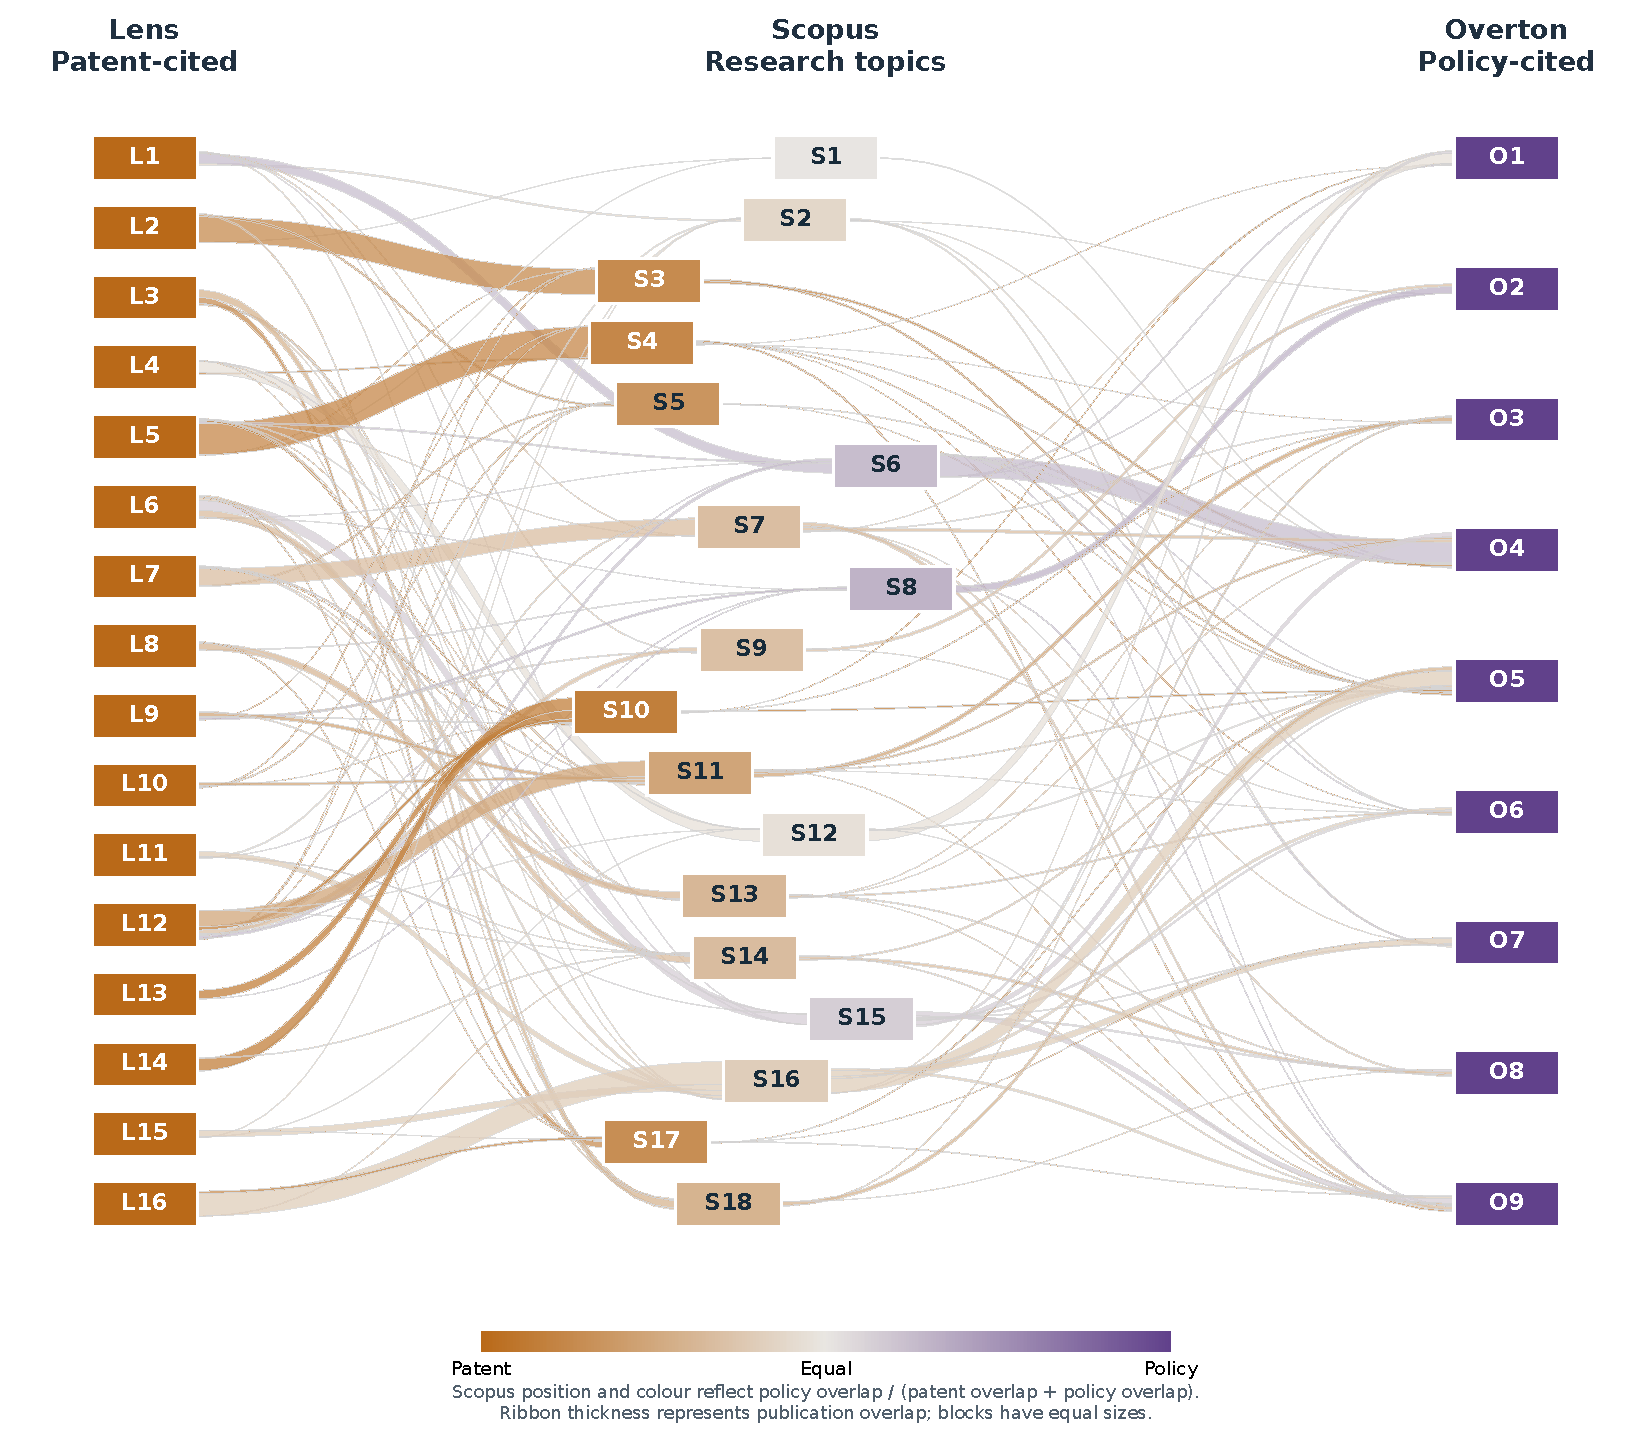
\includegraphics[width=\textwidth,height=0.78\textheight,keepaspectratio]{figs/opf_three_layer_blocks.pdf}
    \caption{Publication overlaps between Scopus, Lens, and Overton topics. Ribbon thickness represents overlap counts. Scopus block colour and horizontal position indicate the relative balance of patent and policy overlaps, from orange (patent) to purple (policy). Blocks have equal sizes; topic codes correspond to Tables~\ref{tab:opf_scopus_topics}, \ref{tab:opf_cited_topics}, and~\ref{tab:opf_policy_topics}.}
    \label{fig:opf_three_layer}
\end{figure}

\FloatBarrier
\subsection{Research Gaps and Future Directions}\label{subsec:opf_research_gaps}

The topic structure identifies several connected research priorities for ML-assisted OPF. The following discussion synthesises limitations reported in the reviewed publications and distinguishes direct OPF evidence from methods developed for neighbouring applications. Particular attention is given to papers represented in all three lists, spanning distributed optimisation, forecasting, renewable integration, electric vehicles, resilience, and digital energy management. These overlaps indicate shared citation attention rather than demonstrated deployment.

\subsubsection{Quantum Computing for Power-System Optimisation}\label{subsubsec:gaps_quantum}

The quantum-computing literature distinguishes the promise of quantum power-system algorithms from evidence of practical computational advantage. Power-system reviews identify hardware limitations, implementation costs, and the need for reproducible demonstrations on realistic applications \cite{zhou2022quantum,golestan2023quantum}. Quantum-inspired metaheuristics offer a separate route to improving classical search, whereas semiconductor spin-qubit research addresses the hardware foundations rather than OPF solution quality \cite{gharehchopogh2023quantum,burkard2023semiconductor}. For OPF, a useful next step is to benchmark complete quantum--classical workflows, including problem encoding, state preparation, measurement, and classical processing, against competitive classical solvers. Tests should report network size, AC feasibility, solution quality, and total execution time, so that potential acceleration is evaluated at the operational-task level.

\subsubsection{Swarm, Evolutionary, and Multiobjective Optimisation}\label{subsubsec:gaps_metaheuristics}

Foundational computational-intelligence and Pareto-optimisation studies provide the basis for population-based search and the treatment of competing objectives \cite{opfRef010,opfRef008}. The PSO, grey-wolf, and manta-ray reviews identify sensitivity to search design, local stagnation, computational effort, and extensions to discrete or multiobjective problems \cite{del2008particle,opfRef035,opfRef070,shami2022particle}. Power-system applications demonstrate evolutionary dispatch, hybrid global--local search, reactive-power optimisation, and FACTS placement, but their results depend on the particular formulation and test conditions \cite{opfRef004,opfRef005,opfRef006,opfRef007,opfRef014,opfRef017}. Future OPF comparisons should therefore use common physical constraints, stopping criteria, and computational budgets, report variability across runs, and compare feasible objective values with mathematical-programming baselines. Learning-based parameter adaptation and warm starts are promising directions, provided their training and evaluation costs are included.

\subsubsection{Physics-Informed and Graph-Based Neural OPF}\label{subsubsec:gaps_neural_opf}

Scientific-ML research motivates incorporating physical knowledge into learned models; engineering model updating, inverse-designed computing structures, and plasmonic manipulation illustrate neighbouring methodological developments rather than demonstrated OPF solutions \cite{willard2022integrating,opfRef016,opfRef056,opfRef088}. Direct OPF studies investigate neural surrogates, graph-based prediction, and feasibility recovery, while related work accelerates building control and security-constrained unit commitment \cite{zamzam2020learning,opfRef071,opfRef082,opfRef041,xavier2021learning}. The reviewed PINN and GNN surveys identify verification, changing network topology, transferability, mixed discrete--continuous decisions, and suitable benchmarks as research needs; empirical GNN scaling laws also require validation across architectures and tasks \cite{huang2022applications,liao2021review,zhu2024scaling,farea2024understanding}. Future OPF models should combine topology-aware learning with explicit feasibility checks or correction, and be tested on unseen networks, loading conditions, and contingencies. Reported acceleration should include correction and solver time, with constraint residuals and optimality gaps reported separately from prediction errors. General MINLP methods remain relevant when extending these models to discrete operating decisions \cite{opfRef020}.

\subsubsection{Reinforcement Learning for Secure Grid Operation}\label{subsubsec:gaps_reinforcement}

The reinforcement-learning reviews identify safety, robustness, sample efficiency, and scalability as barriers to power-system deployment \cite{opfRef073,chen2022reinforcement}. Emergency-control research explicitly proposes larger systems, continuous actions, and safe exploration, while multi-agent theory highlights difficulties arising from partial observability and interactions among learning agents \cite{opfRef064,opfRef085}. For OPF-related control, future work should examine whether actions remain feasible throughout operation, rather than evaluating only cumulative reward or average operating cost. Model-based constraints, safety filters, and conventional-controller fallbacks should be evaluated under changing renewable output, unavailable measurements, and unfamiliar disturbances. Comparable simulation environments and hardware-based tests would help establish when reinforcement learning offers benefits over optimisation-based control.

\subsubsection{Smart-Energy Management and Digital Twins}\label{subsubsec:gaps_digital_twins}

The smart-energy literature links probabilistic ML, renewable integration, and climate-related applications, while emphasising the importance of reliable data and collaboration with operational stakeholders \cite{ahmad2022data,opfRef084,rolnick2022tackling}. IoT and digital-twin studies add challenges concerning resource allocation, communication, modelling interconnected systems, and maintaining correspondence between physical assets and digital representations \cite{opfRef032,opfRef089,thelen2022comprehensive}. These papers have relevance across the research, patent-cited, and policy-cited collections, but their breadth does not itself establish an operational OPF benefit. Future digital-twin studies should connect measurement updates and parameter estimation to a specified OPF decision, and quantify whether this improves feasibility, operating cost, or response time. Validation should include model drift, communication delays, and the computational resources required to keep the twin current.

\subsubsection{Load and Renewable-Generation Forecasting}\label{subsubsec:gaps_forecasting}

Reviews of load forecasting and photovoltaic AI identify opportunities in input selection, hybrid modelling, and uncertainty representation \cite{raza2015review,mellit2008artificial}. The weather-based PV study reports difficulty during typhoon conditions, while the GAN scenario-generation study proposes linking generated scenarios to probabilistic forecasting and operational decision-making \cite{opfRef023,chen2018model}. Broader forecasting studies likewise emphasise probabilistic products tailored to the user's decision problem \cite{opfRef062,petropoulos2022forecasting}. For ML-assisted OPF, the priority is to assess forecasting methods through the decisions they support: reserve procurement, congestion management, curtailment, and constraint violations. Forecasts and scenarios should be evaluated under extreme weather and distribution shifts, preserving relevant spatial and temporal dependence. Lower forecasting error should be tested for operational benefit rather than assumed to imply better OPF performance.

\subsubsection{Grid Resilience and Security Assessment}\label{subsubsec:gaps_resilience}

The resilience and cascading-failure reviews identify the need for consistent resilience metrics, coordinated protection, realistic event models, and assessment across multiple hazards \cite{opfRef031,haes2019survey}. Microgrid studies further highlight uncertain disruption duration, simplified storage dynamics, and the risk that short scheduling horizons inadequately protect future critical demand \cite{opfRef057,opfRef078}. Decision-tree control and security-assessment studies provide methods for representing operating boundaries, while renewable-rich stability reviews discuss changing dynamics and practical implementation \cite{opfRef015,zhang2022data,ali2025power}. Future resilience-oriented OPF should integrate probabilistic hazards, critical-load priorities, restoration constraints, and multi-period resource availability. Learned security boundaries should be checked against appropriate physical simulations and reassessed when network configurations or inverter controls change; economic dispatch feasibility alone is insufficient evidence of dynamic security.

\subsubsection{Cybersecurity and Attack-Resilient OPF}\label{subsubsec:gaps_cybersecurity}

False-data detection demonstrates how learning can distinguish compromised measurements, but detection performance depends on the relationship between attack signatures and measurement noise \cite{opfRef037}. Cyber-physical and smart-grid security reviews identify needs for integrated cyber--physical modelling, contingency analysis, and realistic test environments \cite{opfRef067,ghiasi2023comprehensive}. The resulting OPF research direction is to connect attack detection with the estimation and dispatch decisions affected by corrupted information. Evaluations should include coordinated attacks, unseen attack patterns, detection delay, and false alarms, and measure their consequences for constraint satisfaction and corrective operating cost. Joint assessment of sensing, communication, detection, and optimisation would provide stronger evidence than classification accuracy alone.

\subsubsection{State Estimation, Monitoring, and Fault Diagnosis}\label{subsubsec:gaps_state_estimation}

Voltage-stability analyses establish the importance of load dynamics and reactive-power limitations, while topology identification and learning-based estimation address the information available for operational decisions \cite{opfRef002,opfRef003,bolognani2013identification,opfRef053,opfRef072}. Reviews of clustering and physics-informed reliability modelling identify opportunities in method selection, data availability, and the integration of prior knowledge \cite{miraftabzadeh2023k,xu2023physics}. Feature extraction, turbine diagnosis, and transmission-line inspection provide adjacent diagnostic methods, although their application-specific findings cannot be transferred directly to OPF \cite{opfRef027,opfRef049,opfRef080}. Future work should propagate estimation uncertainty, missing measurements, and topology errors into OPF inputs and constraints. Joint designs for sensor placement, state estimation, and dispatch should assess both computational cost and the reliability of downstream operating decisions, including when diagnostic models encounter unfamiliar equipment conditions.

\subsubsection{Electric-Vehicle Charging and Grid Integration}\label{subsubsec:gaps_ev}

Vehicle--grid integration and smart-charging reviews describe bidirectional-flow, infrastructure, and coordination challenges \cite{opfRef029,sadeghian2022comprehensive}. Vehicle energy-management studies add driving-condition uncertainty, battery limitations, and the need for adaptable real-time strategies \cite{opfRef028,opfRef048,opfRef063}. Converter and on-board-charger reviews show that achievable charging services also depend on efficiency, thermal design, and hardware capability \cite{safayatullah2022comprehensive,opfRef077}. Future charging-aware OPF should jointly represent feeder constraints, uncertain vehicle availability, charging deadlines, battery degradation, and conversion losses. Learning-based charging policies should be compared with stochastic or predictive optimisation under the same information assumptions, and validated across fleet sizes and network conditions. Vehicle-level improvements should be distinguished from demonstrated reductions in grid congestion or operating cost.

\subsubsection{Microgrid, Converter, and Voltage Control}\label{subsubsec:gaps_microgrid_control}

Microgrid-control reviews identify unresolved coordination, communication, convergence, and stability questions \cite{opfRef030,shirkhani2023review}. Converter-control and terminal-sliding-mode studies additionally discuss sensing requirements, disturbance rejection, chattering, and observer design \cite{opfRef074,opfRef075}. Renewable-grid reviews stress reactive-power capability and the interaction of voltage, frequency, and power-quality objectives \cite{opfRef047,opfRef055}. These findings motivate tighter coordination between OPF setpoints and the local controllers that implement them. Future studies should verify that economically selected operating points remain attainable under converter limits and network disturbances, including transitions between grid-connected and islanded operation. Multi-timescale tests should explicitly assess the interaction between optimisation updates, communication delays, and fast control dynamics.

\subsubsection{Uncertainty-Aware Power-System Optimisation}\label{subsubsec:gaps_uncertainty}

Scenario-based microgrid scheduling and probabilistic demand-response studies illustrate the dependence of operating decisions on uncertainty representations \cite{opfRef018,opfRef036}. Reviews of stochastic optimisation and data-driven mathematical programming identify trade-offs among model fidelity, risk representation, computational tractability, and online adaptation \cite{opfRef076,opfRef059,roald2023power}. For OPF, future research should compare stochastic, robust, and distributionally robust formulations using common out-of-sample conditions, rather than treating their uncertainty assumptions as interchangeable. Rare events, correlated renewable shortfalls, and longer time horizons require particular attention. Learned uncertainty sets, scenario reduction, and decision-focused forecasting should be assessed through realised operating costs and violation probabilities, with higher-fidelity AC evaluation used to test the consequences of approximations.

\subsubsection{Storage, Distributed Generation, and Renewable-System Planning}\label{subsubsec:gaps_storage_planning}

Distributed-generation allocation studies show that siting decisions interact with losses, voltage, reliability, and load models; renewable-planning reviews and joint EV--generation allocation further demonstrate the importance of coordinated investment decisions \cite{opfRef009,opfRef013,opfRef021,opfRef038,opfRef040}. Storage and hybrid-renewable reviews call for realistic constraints and consideration of economic, environmental, and operational objectives \cite{opfRef079,opfRef083,worku2022recent,thirunavukkarasu2023comprehensive}. Microgrid MPC explicitly identifies state estimation, uncertainty, and reactive power as extensions, while PV-integration and flexibility reviews highlight network constraints and the need for realistic operational evaluation \cite{opfRef022,shafiullah2022grid,opfRef034}. Future planning models should link investment choices to multi-period OPF, battery ageing, renewable variability, and flexibility provision. ML surrogates can reduce repeated operational calculations, but their approximation errors should be checked for effects on selected capacities, locations, and long-term costs.

\subsubsection{Distributed, Privacy-Preserving, and Integrated-Energy Optimisation}\label{subsubsec:gaps_distributed}

The distributed-optimisation surveys identify practical tuning, time-varying constraints, and coordination of heterogeneous resources as research needs; ADMM convergence results depend on assumptions that must be checked for the implemented formulation \cite{opfRef001,opfRef050,opfRef044}. Reactive-power coordination, network partitioning, and TSO--DSO optimisation illustrate the importance of decomposition and information exchange \cite{opfRef025,opfRef046,opfRef043}. Integrated electricity--gas and electricity--heat studies add coupled dynamics, uncertainty, and computational trade-offs \cite{opfRef039,opfRef042,opfRef086}. Blockchain-based energy coordination and edge-computing studies raise further questions about scalability, security, and execution speed \cite{opfRef033,opfRef054,opfRef065,opfRef081}. Future ML-assisted distributed OPF should evaluate learned warm starts or coordination rules under realistic communication budgets and incomplete information. Testing should retain feasibility and convergence checks, and distinguish limited data exchange from a demonstrated privacy guarantee.

\subsubsection{Peer-to-Peer Markets and Network-Constrained Coordination}\label{subsubsec:gaps_markets}

Multi-microgrid trading and community-market studies connect decentralised optimisation with participant preferences, while market reviews identify asynchronous communication, strategic behaviour, and scalability as research directions \cite{opfRef024,sousa2019peer,opfRef087}. Product differentiation and multi-class trading studies explicitly question how participant behaviour and larger market participation affect coordination, and coordinated market design demonstrates why energy transactions must respect physical network constraints \cite{opfRef052,opfRef058,opfRef066}. Future OPF-linked market mechanisms should jointly examine congestion, losses, voltage limits, ancillary services, and settlement incentives. ML forecasts or bidding policies should be evaluated with heterogeneous and potentially strategic participants, while testing whether market-clearing outcomes remain physically feasible and whether communication requirements remain practical as participation grows.

\section{Conclusions}\label{sec:conclusions}

This study examined the academic, patent-cited, and policy-cited ML--OPF literature through DOI linkage, bibliometric analysis, and independently estimated topic models. Among 15,857 DOI-linked publications, 778 received patent citations and 392 received policy citations, with 83 shared between the two collections. Patent citations therefore reached a larger publication set, while policy citations were more concentrated among the publications they reached. The limited publication-level overlap supports examining both pathways when assessing external research attention.

The thematic analysis identified 18 Scopus, 16 Lens, and nine Overton topics. Patent-cited research included specific computational approaches, particularly reinforcement learning, neural OPF surrogates, and distributed optimisation. Policy-cited research grouped publications more broadly around energy-system management, grid resilience, renewable integration, and network-constrained coordination. Neural learning for OPF and reinforcement learning increased their shares of the academic literature, whereas established distributed and metaheuristic optimisation themes declined in relative share. Distributed optimisation nevertheless remained a substantial research topic with connections across both external citation pathways. These findings show that research volume, thematic growth, and external citation coverage describe different aspects of the ML--OPF knowledge base.

The literature synthesis identifies several priorities for future research: verifying physical feasibility and solution quality, evaluating generalisation across networks and operating conditions, connecting forecasting improvements to operational decisions, and testing distributed methods under realistic communication and information constraints. Progress should be assessed through reproducible comparisons that include correction costs, uncertainty, contingencies, and implementation requirements. Such evaluation can clarify when ML provides an operational advantage over established optimisation methods.

The findings are bounded by the broad Scopus search, DOI-based matching, database coverage, interpretive topic labels, and unequal citation-accumulation periods. Repeated-seed stability was not established for the retained topic models. Patent and policy citations indicate documented attention rather than demonstrated commercialisation, adoption, or causal influence. Within these limits, the combined framework provides a basis for identifying shared research foundations and differences between invention-oriented and policy-oriented attention to ML--OPF research.

% \section*{Declaration of generative AI and AI-assisted technologies in the writing process}

% \section*{Funding}
% This research \& publication is supported by the Interdisciplinary Research Center for Intelligent Secure Systems under Project \# INSS2620. 

\section*{Acknowledgements}
The authors would like to acknowledge all support provided by Interdisciplinary Research Center for Intelligent Secure Systems and Department of Industrial and Systems Engineering, at King Fahd University of Petroleum and Minerals (KFUPM).

%% Loading bibliography style file
%\bibliographystyle{model1-num-names}
\bibliographystyle{cas-model2-names}

% Loading bibliography database
% \bibliography{cas-refs}
\bibliography{cas-refs_OPF_updated}

%\vskip3pt

% \bio{}
% Author biography without author photo.
% Author biography. Author biography. Author biography.
% Author biography. Author biography. Author biography.
% Author biography. Author biography. Author biography.
% Author biography. Author biography. Author biography.
% Author biography. Author biography. Author biography.
% Author biography. Author biography. Author biography.
% Author biography. Author biography. Author biography.
% Author biography. Author biography. Author biography.
% Author biography. Author biography. Author biography.
% \endbio

% \bio{figs/cas-pic1}
% Author biography with author photo.
% Author biography. Author biography. Author biography.
% Author biography. Author biography. Author biography.
% Author biography. Author biography. Author biography.
% Author biography. Author biography. Author biography.
% Author biography. Author biography. Author biography.
% Author biography. Author biography. Author biography.
% Author biography. Author biography. Author biography.
% Author biography. Author biography. Author biography.
% Author biography. Author biography. Author biography.
% \endbio

% \bio{figs/cas-pic1}
% Author biography with author photo.
% Author biography. Author biography. Author biography.
% Author biography. Author biography. Author biography.
% Author biography. Author biography. Author biography.
% Author biography. Author biography. Author biography.
% \endbio

\end{document}

